\documentclass{article}

\usepackage[main=english,vietnamese]{babel}
\usepackage[T1]{fontenc}
\usepackage[utf8]{inputenc}
\usepackage[sexy]{evan}
\usepackage{matchsticks}
\usepackage{wrapfig}
\usepackage{listings}

\newtheorem{hint}{Hint}

\title{Derivative II}
\author{Nghia Doan}
\date{\today}

\begin{document}

\maketitle

\begin{problem*}[1a]
    We restrict the function $\sec(x)$ on $\left[ 0, \frac{\pi}{2} \right) \cup \left[ \pi, \frac{3\pi}{2} \right)$ to get an one-to-one function.
    We call it $f(x).$ We define the inverse of this function be $f^{-1}(x).$

    Find the domain and range of $f^{-1}.$
\end{problem*}

\begin{soln}
    The domain of $f^{-1}$ is $\left( -\infty, -1 \right] \cup \left[ 1, +\infty \right).$
    The range of $f^{-1}$ is $\left[ 0, \frac{\pi}{2} \right) \cup \left[ \pi, \frac{3\pi}{2} \right).$
\end{soln}

\begin{problem*}[1b]
    Compute $f^{-1}(sec(5))$ and $sec(f^{-1}(5)).$
\end{problem*}

\begin{soln}
    $f^{-1}(sec(5)) = 1.28,\ sec(f^{-1}(5)) = 5.$
\end{soln}

\begin{problem*}[1c]
    Sketch the graph of $\sec \circ f^{-1}.$ Make sure to label your axes and that you have the correct domain.
\end{problem*}

\begin{center}
    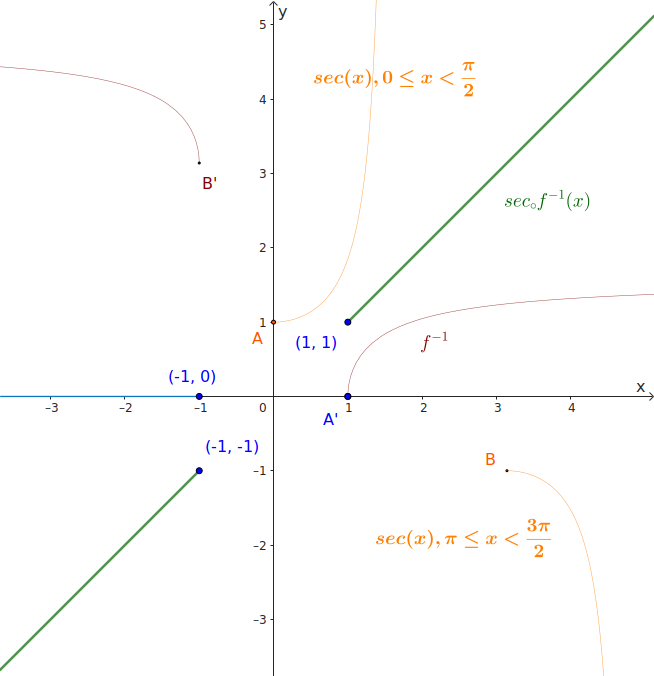
\includegraphics[width=10cm]{./svg/pdf/derivative-2-1c-f.pdf}
\end{center}

\begin{soln}
    Both the domain and the range of $\sec \circ f^{-1}$ are the same: $(-\infty, -1] \cup [+1, +\infty).$

    $\sec \circ f^{-1}(x) = x,\ \forall x \in (-\infty, -1] \cup [+1, +\infty).$
\end{soln}

\newpage

\begin{problem*}[1d]
    Sketch the graph of $f^{-1} \circ \sec.$ Make sure to label your axes and that you have the correct domain.
\end{problem*}

\begin{center}
    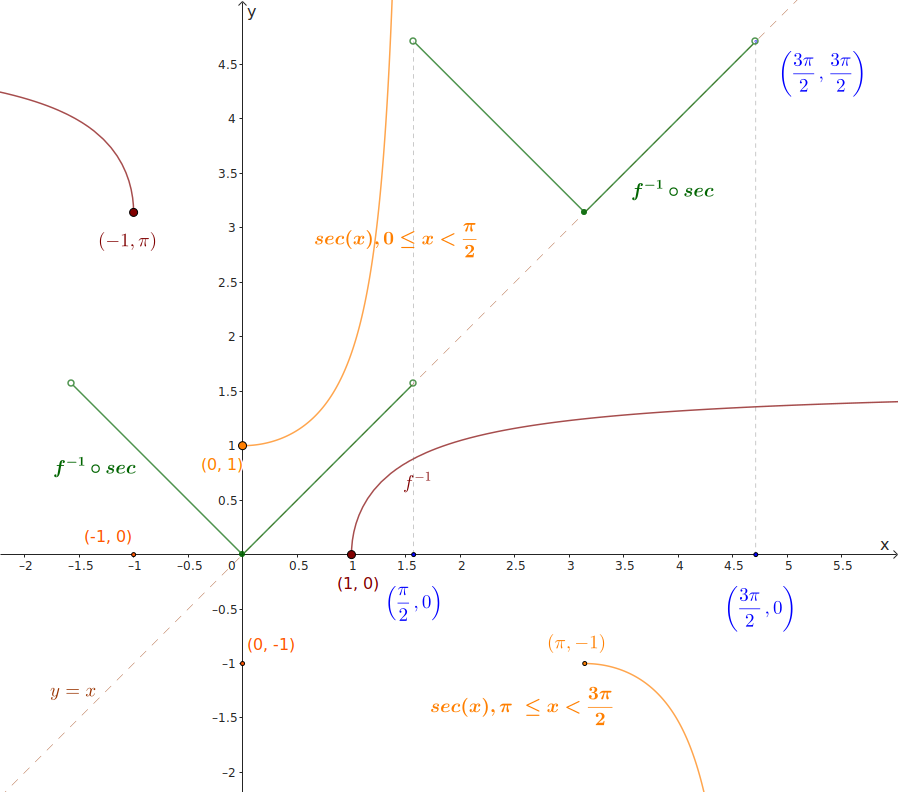
\includegraphics[width=14cm]{./svg/pdf/derivative-2-1d-f.pdf}
\end{center}

\begin{soln}
    $f^{-1} \circ \sec:\ \RR \setminus \{ \frac{\pi}{2} + k \pi \mid k \in \ZZ \} \rightarrow \left[0, \frac{\pi}{2} \right) \cup \left[\pi, \frac{3\pi}{2} \right)$:
    \[
        (f^{-1} \circ \sec)(x) = 
        \left\{
            \begin{aligned}
                -x + 2k\pi, &\ \forall x \in \left( -\frac{\pi}{2} + 2k\pi,\ 2k\pi \right]\\
                x - 2k\pi, &\ \forall x \in \left[ 2k\pi,\ \frac{\pi}{2} + 2k\pi \right)\\
                -x + 2(k+1)\pi, &\ \forall x \in \left( \frac{\pi}{2} + 2k\pi,\ \pi + 2k\pi \right]\\
                x - 2k\pi, &\ \forall x \in \left[ \pi + 2k\pi,\ \dfrac{3\pi}{2} + 2k\pi \right)
            \end{aligned}
        \right.
    \]
\end{soln}

\newpage

\begin{problem*}[1e]
    Find a formula for the derivative of $f^{-1}.$
\end{problem*}

\begin{soln}
    Let $I_1 = \left( -\infty, -1 \right] \cup \left[ 1, +\infty \right),$ $I_2 = \left[ 0, \frac{\pi}{2} \right) \cup \left[ \pi, \frac{3\pi}{2} \right),$
    \[
        y:\ I_1 \rightarrow I_2: y(x) = f^{-1}(x) \Rightarrow y(x) = \sec^{-1}(x) \Rightarrow \sec(y(x)) = x \quad (*)
    \]

    $\forall x \in \left[ 0, \frac{\pi}{2} \right) \cup \left[ \pi, \frac{3\pi}{2} \right):$
    \[
        \begin{aligned}
            &\frac{d}{dx} \sec(x) = \frac{d}{dx} \frac{1}{\cos{x}} = - \frac{1}{(\cos{x})^2} \cdot \frac{d}{dx} \cos(x)
            = - \frac{1}{(\cos{x})^2} \cdot (- \sin{x}) =  \frac{1}{\cos{x}} \cdot \frac{\sin{x}}{\cos{x}} = \sec(x) \tan(x).\\
        \end{aligned}
    \]

    $\forall x \in \left( -\infty, -1 \right] \cup \left[ 1, +\infty \right):$
    \[
        sec(y(x)) = x \Rightarrow \frac{d}{dx} \sec(y(x)) = \frac{d}{dx} (x) 
        \Rightarrow \sec(y(x)) \tan(y(x)) \cdot \frac{dy(x)}{dx} = 1 \quad (**)
    \]

    $\forall x \in \left( -\infty, -1 \right) \cup \left( 1, +\infty \right):$
    \[
        \begin{aligned}
            &x \in \left( -\infty, -1 \right) \Rightarrow y(x) \in \left( \pi, \frac{3\pi}{2} \right) \Rightarrow \cos{y(x)} < 0, \sin{y(x)} < 0 \Rightarrow \tan(y(x)) > 0\\
            &x \in \left( +1, +\infty \right) \Rightarrow y(x) \in \left( 0, \frac{\pi}{2} \right) \Rightarrow \cos{y(x)} > 0, \sin{y(x)} > 0 \Rightarrow \tan(y(x)) > 0\\
            &\Rightarrow \tan(y(x)) > 0 \quad (***)
        \end{aligned}        
    \]

    $\forall x \in \left( -\infty, -1 \right) \cup \left( 1, +\infty \right),$ from (*), (**), and (**):
    \[
        \begin{aligned}
            &\tan^2(y(x)) = \frac{\sin^2(y(x))}{\cos^2(y(x))} = 1- \dfrac{1}{\cos^2(y(x))} = 1 - \sec^2(y(x))\\
            &\frac{d y(x)}{dx} = \frac{1}{\sec(y(x)) \tan(y(x))} = \frac{1}{\sec(y(x)) \sqrt{1-\sec^2(y(x))}} = \frac{1}{x \sqrt{1-x^2}}.
        \end{aligned}
    \]

    Hence, $\forall x \in \left( -\infty, -1 \right) \cup \left( 1, +\infty \right),$ 
    \[
        \frac{d f^{-1}(x)}{dx} = \frac{1}{x \sqrt{1-x^2}}.
    \]
\end{soln}

\newpage

\begin{problem*}[2a]
    Let $a<b$ and $f$ be a function defined on $[a,b].$ Suppose that $f$ is a continuous function on $[a,b]$, and $f$ is differentiable on $(a,b)$, 

    Let $x \in \left[ a, b \right)$ and let $h > 0$ be such that $x+h \le b.$ Prove that there is $\theta \in (0,1)$ such that:
    \[
        \frac{f(x+h) - f(x)}{h} = f'(x+\theta h).
    \]
\end{problem*}

\begin{soln}
    First, $f$ is a continuous function on $[a,b]$, and $f$ is differentiable on $(a,b)$, and $[x, x+h] \subseteq [a,b],$
    therefore $f$ is continuous on $[x, x+h]$ and $f$ is differentiable on $(x, x+h).$ 

    Second, by the Mean-Value Theorem for $f$ is continuous on $[x, x+h],$ $f$ is differentiable on $(x, x+h),$ there exists $c \in (x, x+h),$ such that:
    \[
        f'(c) = \frac{f(x+h)-f(x)}{(x+h) - x} = \frac{f(x+h) - f(x)}{h}.
    \]

    By choosing $\theta = \dfrac{c-x}{h},$ then
    \[
        \begin{aligned}
            &c > x \Rightarrow \theta > \frac{x-x}{h} = 0,\ c < x+h \Rightarrow \theta < \frac{(x+h)-x}{h} = 1 \Rightarrow \theta \in (0, 1),\ \text{and}\\
            &x + \theta h = x + \dfrac{c-x}{h}  = c \Rightarrow f'(x+ \theta h) = \frac{f(x+h) - f(x)}{h}.
        \end{aligned}
    \]

    Hence, there exists $\theta \in (0,1)$ such that, 
    \[
        \frac{f(x+h) - f(x)}{h} = f'(x + \theta h).
    \]
\end{soln}

\bigbreak

\begin{problem*}[2b]
    Consider $f(y) = \ln(y).$ Fix $x >0$ and $h>0.$ Find $\theta$ in term of $x$ and $h,$ as in the previous formula.
\end{problem*}

\begin{soln}
    $x > 0, h > 0,$ $f(x)=\ln(x)$ is a continuous function on $[x,x+h]$, and is differentiable on $(x, x+h).$

    Note that $\ln(x+h) \ne \ln(x),$ by result of (2a), there exists $\theta \in (0,1)$  such that
    \[
        \begin{aligned}
            &\frac{f(x+h) - f(x)}{h} = f'(x + \theta h) \Rightarrow (\ln(x + \theta h))' = \frac{\ln(x+h) - \ln(x)}{h}\\
            &\Rightarrow \frac{1}{x + \theta h} = \frac{\ln(x+h) - \ln(x)}{h} \Rightarrow x + \theta h = \frac{h}{\ln(x+h) - \ln(x)}\\
            &\Rightarrow \theta = \boxed{\frac{h - x \ln(x+h) + x \ln(x)}{h(\ln(x+h) - \ln(x))}.}
        \end{aligned}
    \]
\end{soln}

\newpage

\begin{problem*}[2c]
    Fix $x >0.$ Find
    \[
        \lim_{h \rightarrow 0} \theta(x,h)
    \]
\end{problem*}

\begin{soln}
    From the result from (2b), for $x > 0, h > 0:$ 
    \[
        \theta(x,h) = \frac{h - x \ln(x+h) + x \ln(x)}{h(\ln(x+h) - \ln(x))} = \frac{ h - x \ln(x+h) + x \ln(x) }{h^2} \cdot \frac{h}{\ln(x+h) - \ln(x)}
    \]

    By L'Hopital rule,
    \[
        \lim_{h \rightarrow 0} \frac{ h - x \ln(x+h) + x \ln(x) }{h^2} = \lim_{h \rightarrow 0 } \frac{\frac{d}{dh} (h - x \ln(x+h) + x \ln(x))}{\frac{d}{dh} h^2}
        = \lim_{h \rightarrow 0 } \frac{1 - \frac{x}{x+h}}{2h} = \lim_{h \rightarrow 0 } \frac{1}{2(x+h)} = \frac{1}{2x}.
    \]

    On the other hand, for $x >0:$
    \[
        \lim_{h \rightarrow 0} \frac{h}{\ln(x+h) - \ln(x)} = \frac{1}{(\ln (x))'} = x.
    \]

    Thus,
    \[
        \lim_{h \rightarrow 0} \theta(x,h) = \frac{1}{2x} \cdot x = \boxed{\frac{1}{2}}
    \]
\end{soln}

\newpage

\begin{problem*}[3a]
    Suppose that $f$ is continuous on $[a,b]$ and that $a < f(x) < b$ for all $x \in [a,b].$
    Prove that there exists $c \in (a, b)$ such that $c = f(c).$ 
    \textit{Hint: Consider the function $g(x) = x - f (x).$}
\end{problem*}

\begin{soln}
    Consider the function $g: [a,b] \rightarrow \RR: g(x) = x - f(x),$
    then $g$ is continuous on $(a,b),$ $g(a) = a - f(a) < 0$ and $g(b) = b - f(b) > 0.$
    By the Intermediate-Value Theorem, there exits $c \in (a,b)$ such that $g(c) = 0,$ or $\boxed{c = f(c).}$
\end{soln}

\bigbreak

\begin{problem*}[3b]
    Suppose, in addition, that $f$ is differentiable on $(a,b)$ and that $|f'(x)| < 1$ for all $x \in (a,b).$
    Prove that there is a unique point $c \in (a, b)$ such that $c = f(c).$
    \textit{Hint: Use MVT.}
\end{problem*}

\begin{soln}
    From (3a) there exists a $c \in (a,b)$ such that $c = f(c).$
    We prove that $c$ is the only value in $(a,b)$ such that $c = f(c).$
    Assume the contrary, then exists $c_1 \in (a,b), c_1 \ne c,$ such that $c_1 = f(c_1).$ 
    
    Since the roles of $c$ and $c_1$ are the same, so without loss of generality, let's assume that $c < c_1.$

    $f$ is continuous on $[a,b],$ $f$ is differentiable on $(a,b),$ and since $a < c < c_1 < b,$
    thus $f$ is continuous on $[c,c_1],$ and $f$ is differentiable on $(c,c_1).$
    
    By the Mean-Value Theorem there exists some real number $d \in (c,c_1)$ such that 
    \[
        f'(d) = \frac{f(c_1) - f(c)}{c_1 - c}.
    \]

    Then $f(c_1) = c1, f(c) = c, c\ne c_1,$ thus $f'(d) = 1.$
    However $|f'(x)| < 1,\ \forall x \in (a,b),$ $(c,c_1) \subseteq (a,b),$ so $|f'(x)| < 1,\ \forall x \in (c, c_1),$
    this is a contraction to the existence of $d \in (a,b)$
    
    (*) contradicts (**), the assumption was wrong.
    Hence, $c$ is the only value in $(a,b)$ such that $c = f(c).$
\end{soln}

\newpage

\begin{problem*}[3c]
    Using parts (a) and (b), show that the equation $\tan(3x) = \sqrt{2x + 1}$ has a unique solution on $(0, 1).$
    \textit{Formulate this equation as $x = f(x)$ for some function $f(x).$ Then use the results from part (a) and part (b)}
\end{problem*}

\begin{soln}
    First, we prove that the equation $\tan(3x) = \sqrt{2x + 1}$ has a solution on $(0, 1).$
    
    Note that $\cos(3(\frac{\pi}{6})) = 0,$ so $\tan(3x)$ does not exist if $x = \frac{pi}{6}.$

    Let $f: \left[0,  1 \right] \setminus \{ \frac{pi}{6} \} \rightarrow \RR:$
    \[
        f(x) = \tan(3x) - \sqrt{2x + 1}.
    \]

    \[
        \begin{cases}
            &0.5 < \frac{\pi}{6} \approx 0.52,\ \tan(3\cdot 0.5) - \sqrt{2*0.5+1} \approx 12.68\\
            &\tan(0)- \sqrt{2\cdot 0 + 1} = -1.
        \end{cases}
    \]

    $f$ is continuous on $[0, 0.5],$ by the Intermediate-Value Theorem, there exists $c \in (0, 0.5),$ such that $f(c) = 0.$
    Therefore $c$ is a solution on $(0,1)$ of the given equation.

    Now, we prove that $c$ is the only solution on $(0,1)$ of the equation $\tan(3x) = \sqrt{2x + 1}.$
    Assume the contrary that there exists some real number $c \in (0, 1)$ such that $\tan(3c) - \sqrt{2c + 1} = 0.$

    The function $f$ is continuous and is differentiable on $\left[0,  1 \right] \setminus \{ \frac{\pi}{6} \},$ its derivative is 
    \[
        f'(x) = \dfrac{3}{\cos^2(3x)} - \dfrac{1}{\sqrt{2x + 1}}.
    \]

    For all $x \in \left[0,  1 \right] \setminus \{ \frac{\pi}{6} \},$ then $3\sqrt{2x + 1} > 3 > \cos^2(3x) > 0,\ $ thus $f'(x) > 0,$ \quad (*)

    \textit{Case 1:} If $c \in \left[0,  \frac{\pi}{6} \right).$ 
    The roles of $c$ and $c_1$ are the same, without loss of generality, let's assume $c < c_1.$
    
    The function $f(x) = \tan(3x) - \sqrt{2x + 1}$ is continuous $\left[0,  \frac{\pi}{6} \right),$ so it is continuous on $(c, c_1).$.
    $f$ is differentiable on $\left[0,  \frac{\pi}{6} \right),$ thus it is differentiable on $(c, c_1).$

    By the Mean-Value Theorem there exists some real number $d \in (c,c_1)$ such that 
    \[
        f'(d) = \frac{f(c_1) - f(c)}{c_1 - c} = 0 \quad (**)
    \]
    
    (**) contradicts (*), thus $c \not \in \left[0,  \frac{\pi}{6} \right)$ \quad (1)  

    \textit{Case 2:} If $c \in \left(\frac{\pi}{6}, 1 \right].$ 
    Note that $f(1) = \tan(3) - \sqrt{3} \approx -1.874 < -1.87.$

    Since $f$ is continuous on $[c_1, 1],$ differentiable on $[c_1, 1],$ by the Mean-Value Theorem there exists some real number $d \in (c_1, 1)$ such that:
    \[
        f'(d) = \frac{f(1) - f(c_1)}{1 - c_1} < \frac{-1.87 - c_1}{1-c_1} < 0 \quad (***)
    \]

    (***) contradicts (*), thus $c \not \in \left(\frac{\pi}{6}, 1 \right]$ \quad (2)
    
    From (1) and (2), there is no such $c_1 \ne c$: $f(c_1) = c_1.$
    Hence, $c$ is a unique solution.
\end{soln}

\newpage

\begin{problem*}[4]
    We are filling water from a conic tank (with vertex down) to a cylindrical tank.
    The conic tank has height 18 m and the radius of the base 6 m. The diameter of the cylindrical tank’s base is 10 m.
    We know the water level in the conic tank is decreasing at 1m/s when the water level is 12 m.
    Find the rate of change of the water level in the cylindrical tank.
\end{problem*}

\begin{soln}
    First, let calculate the volume of the conic tank. It is a (inverted) cone with base radius $r_1 = 6,$ height $h_1 = 18.$
    Therefore its \textit{full} volume is:
    \[
        V_1 = \frac{1}{3} \pi r_1^2 h_1,\text{\ where\ } r_1 : h_1 = 1 : 3.
    \] 

    If we consider $t$ as the variable of time, then $h$ is a function of $t,$ and $r$ can simply be calculated from $h$
    (the height and radius of the cone formed by the water are proportional to $h$ and $r$ by similar triangles):
    \[
        V_1 = \frac{1}{3} \pi r^2 h = \frac{\pi}{3} \left(\frac{1}{3} h \right)^2 h =  \frac{\pi}{27} h^3 \quad (*)
    \]

    When the water level is $12$ ($h = 12$), the change in rate of the water level $h$ in the conic tank is $-1,$ which means that $\dfrac{dh}{dt} = -1.$
    Thus the rate of change in water volume at the time $t$ (when $h=12$) is
    \[
        \frac{dV_1}{dt} = \frac{d}{dt} \left( \frac{\pi}{27} h^3 \right) = \frac{\pi}{9} h^2 \dfrac{dh}{dt} = \frac{\pi}{9} h^2 (-1)
        \Rightarrow \frac{dV_1}{dt} = - \frac{12^2 \pi}{9} = - 16\pi.
    \]

    This is the volume of water discharged from the conic tank into the cylindrical tank under it.
    The water volume that the cylindrical tank received must be the opposite of what the conic tank discharged:
    \[
        \frac{dV_2}{dt} = - \frac{dV_1}{dt} = 16\pi.
    \]

    The cylindrical tank volume function with radius $r_2 = \frac{10}{2}  = 5$ is $V_2 = \pi r_2^2 h,$ therefore:
    \[
        \frac{dV_2}{dt} = 25 \pi \frac{dh}{dt} \Rightarrow 16\pi = 25 \pi \frac{dh}{dt}  \rightarrow \frac{dh}{dt}  = \boxed{\frac{16}{25}} \text{\ m/s.}
    \]
\end{soln}

\newpage

\begin{problem*}[5]
    Let $0 < a < b < 2a.$ We will consider the curve $xy=1$ on $[a,b].$ We now sketch a tangent line at any point $(x,y)$ on this curve with $x-$coordinate in $[a,b].$
    Then we will have a trapezoid and its four sides are on this tangent line, $x-$axis, $x = a$ and $x = b.$
    Find the point $(x, y)$ such that the area of the trapezoid is the largest.
\end{problem*}

\begin{center}
    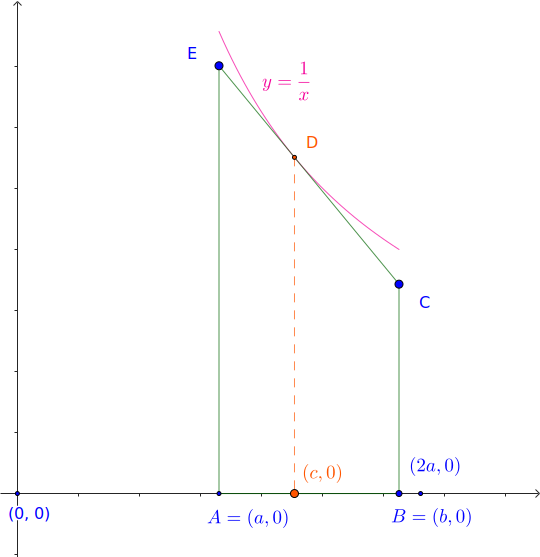
\includegraphics[width=10cm]{./svg/pdf/derivative-2-5.pdf}
\end{center}

\begin{soln}
    Let $D \left(c, \frac{1}{c} \right)$ the point. Then 
    \[
        a < c < b < 2a \Rightarrow a < c < b < 2a < 2c \quad (*)
    \]
    
    The slope of the tangent line is $f'(c) = -\dfrac{1}{c^2},$ thus the equation of the tangent line through $D$ is:
    \[
        y -  \frac{1}{c} = \left( -\frac{1}{c^2} \right) (x-c) \quad (*)
    \]

    Thus $C$ and $E$ coordinates are
    \[
        C \left( b, -\frac{1}{c^2}(b-c) + \frac{1}{c} \right) \text{\ or\ } C\left( b, \frac{2c - b}{c^2} \right),\ 
        E \left( a, -\frac{1}{c^2}(a-c) + \frac{1}{c} \right) \text{\ or\ } E\left( a, \frac{2c - a}{c^2} \right).
    \]

    The distances $BC$ and $AE$:
    \[
        BC = \frac{2c - b}{c^2},\ AE = \frac{2c - a}{c^2}
        \Rightarrow \half(BC + AE) = \half \left( \frac{2c - b}{c^2} + \frac{2c - a}{c^2} \right) = \frac{4c - a - b}{2c^2}
    \]

    Thus the area $[ABCE],$
    \[
        [ABCE] = AB \cdot \half(BC + AE) = (b-a)\frac{4c - a - b}{2c^2}
    \]

    Note that,
    \[
        (2c -a -b)^2 \ge 0 \Leftrightarrow  4c^2 - 4c(a+b) + (a+b)^2 \ge 0 \Leftrightarrow 4c^2 \ge (a+b) (4c-a-b) \Leftrightarrow \frac{2}{a+b} \ge \frac{4c - a - b}{2c^2}
    \]

    Thus 
    \[
        [ABCE] = (b-a)\frac{4c - a - b}{2c^2} \le \frac{2(b-a)}{a+b}.
    \]

    The area of the trapezoid is largest when $(2c -a -b)^2 \ge 0,$ or $c = \frac{a+b}{2}.$
    Hence point $(x,y)$ is $\left(\frac{a+b}{2}, 0\right).$
\end{soln}


\end{document}